

%\documentclass[12pt]{article}
\documentclass[12pt, letterpaper]{book}
\title{CHEM 121: Nomenclature practice}
\nonstopmode
\usepackage{graphicx} % Required for including pictures
\usepackage[figurename=Figure]{caption}
\usepackage{float}    % For tables and other floats
\usepackage{verbatim} % For comments and other
\usepackage{amsmath}  % For math
\usepackage{amssymb}  % For more math
\usepackage{fullpage} % Set margins and place page numbers at bottom center
\usepackage{paralist} % paragraph spacing
\usepackage{listings} % For source code
\usepackage{subfig}   % For subfigures
%\usepackage{physics}  % for simplified dv, and 
\usepackage{wrapfig}
\usepackage{enumitem} % useful for itemization
\usepackage{siunitx}  % standardization of si units

\usepackage{tikz,bm} % Useful for drawing plots
%\usepackage{tikz-3dplot}
\usepackage{circuitikz}
\usepackage{url}
\usepackage[table]{xcolor}
%Settings parameters for how tables will be formatted
\setlength{\arrayrulewidth}{0.5mm}
\setlength{\tabcolsep}{20pt}
%Package to help with formatting chemical formulae
\usepackage[version=4]{mhchem}

\usepackage{fontspec}

\usepackage{titlesec}

\usepackage[paperheight=16cm, paperwidth=12cm,% Set the height and width of the paper
includehead,
nomarginpar,% We don't want any margin paragraphs
textwidth=10cm,% Set \textwidth to 10cm
headheight=10mm]% Set \headheight to 10mm

\usepackage{fancyhdr}

\titleformat{\section}
  {\center\normalfont\normalsize\bfseries}{}{2em}{}
\titleformat{\subsection}
{\normalfont\normalsize\bfseries}{}{1em}{}
\titleformat{\paragraph}
{\normalfont\normalsize\mdseries}{}{0em}{}

\usepackage[skip=12pt plus1pt, indent=0pt]{parskip}


\begin{document}

% Set the page style to "fancy"...
\pagestyle{fancy}
\renewcommand{\headrulewidth}{0pt}
\fancyhead{}
\fancyhead[R]{\thepage}
\fancyfoot{} % clear all footer fields
\renewcommand{\footrulewidth}{0.1pt}
\fancyfoot[L]{Truman Science Center}
\fancyfoot[C]{Introductory Chemical Nomenclature}
\fancyfoot[R]{8 April 2026}

\setmainfont{Arial}[Scale=0.9]
\captionsetup{belowskip=1pt}


\begin{flushleft}
	\vspace{.3cm}
	{\textbf { \Large Introductory Chemistry Nomenclature}}
\end{flushleft}
\vspace{1mm}
	\hrule
    


\section{{\normalsize The Process}}

The first step is always to determine which category the compound fits into because each category has different naming conventions. 

\subsection{{\normalsize Covalent Bonding: nonmetal bound to a nonmetal}}

The nonmetals are elements found in columns 13-18 (also sometimes called columns 3a to 8a) and above the metalloid stair step. Hydrogen is also part of this group. These elements are colored red in the periodic table above. When the compound is only composed of two elements that are both from this part of the periodic table, the number of atoms of each element is denoted with a prefix.

\begin{figure}[H]
    \centering
    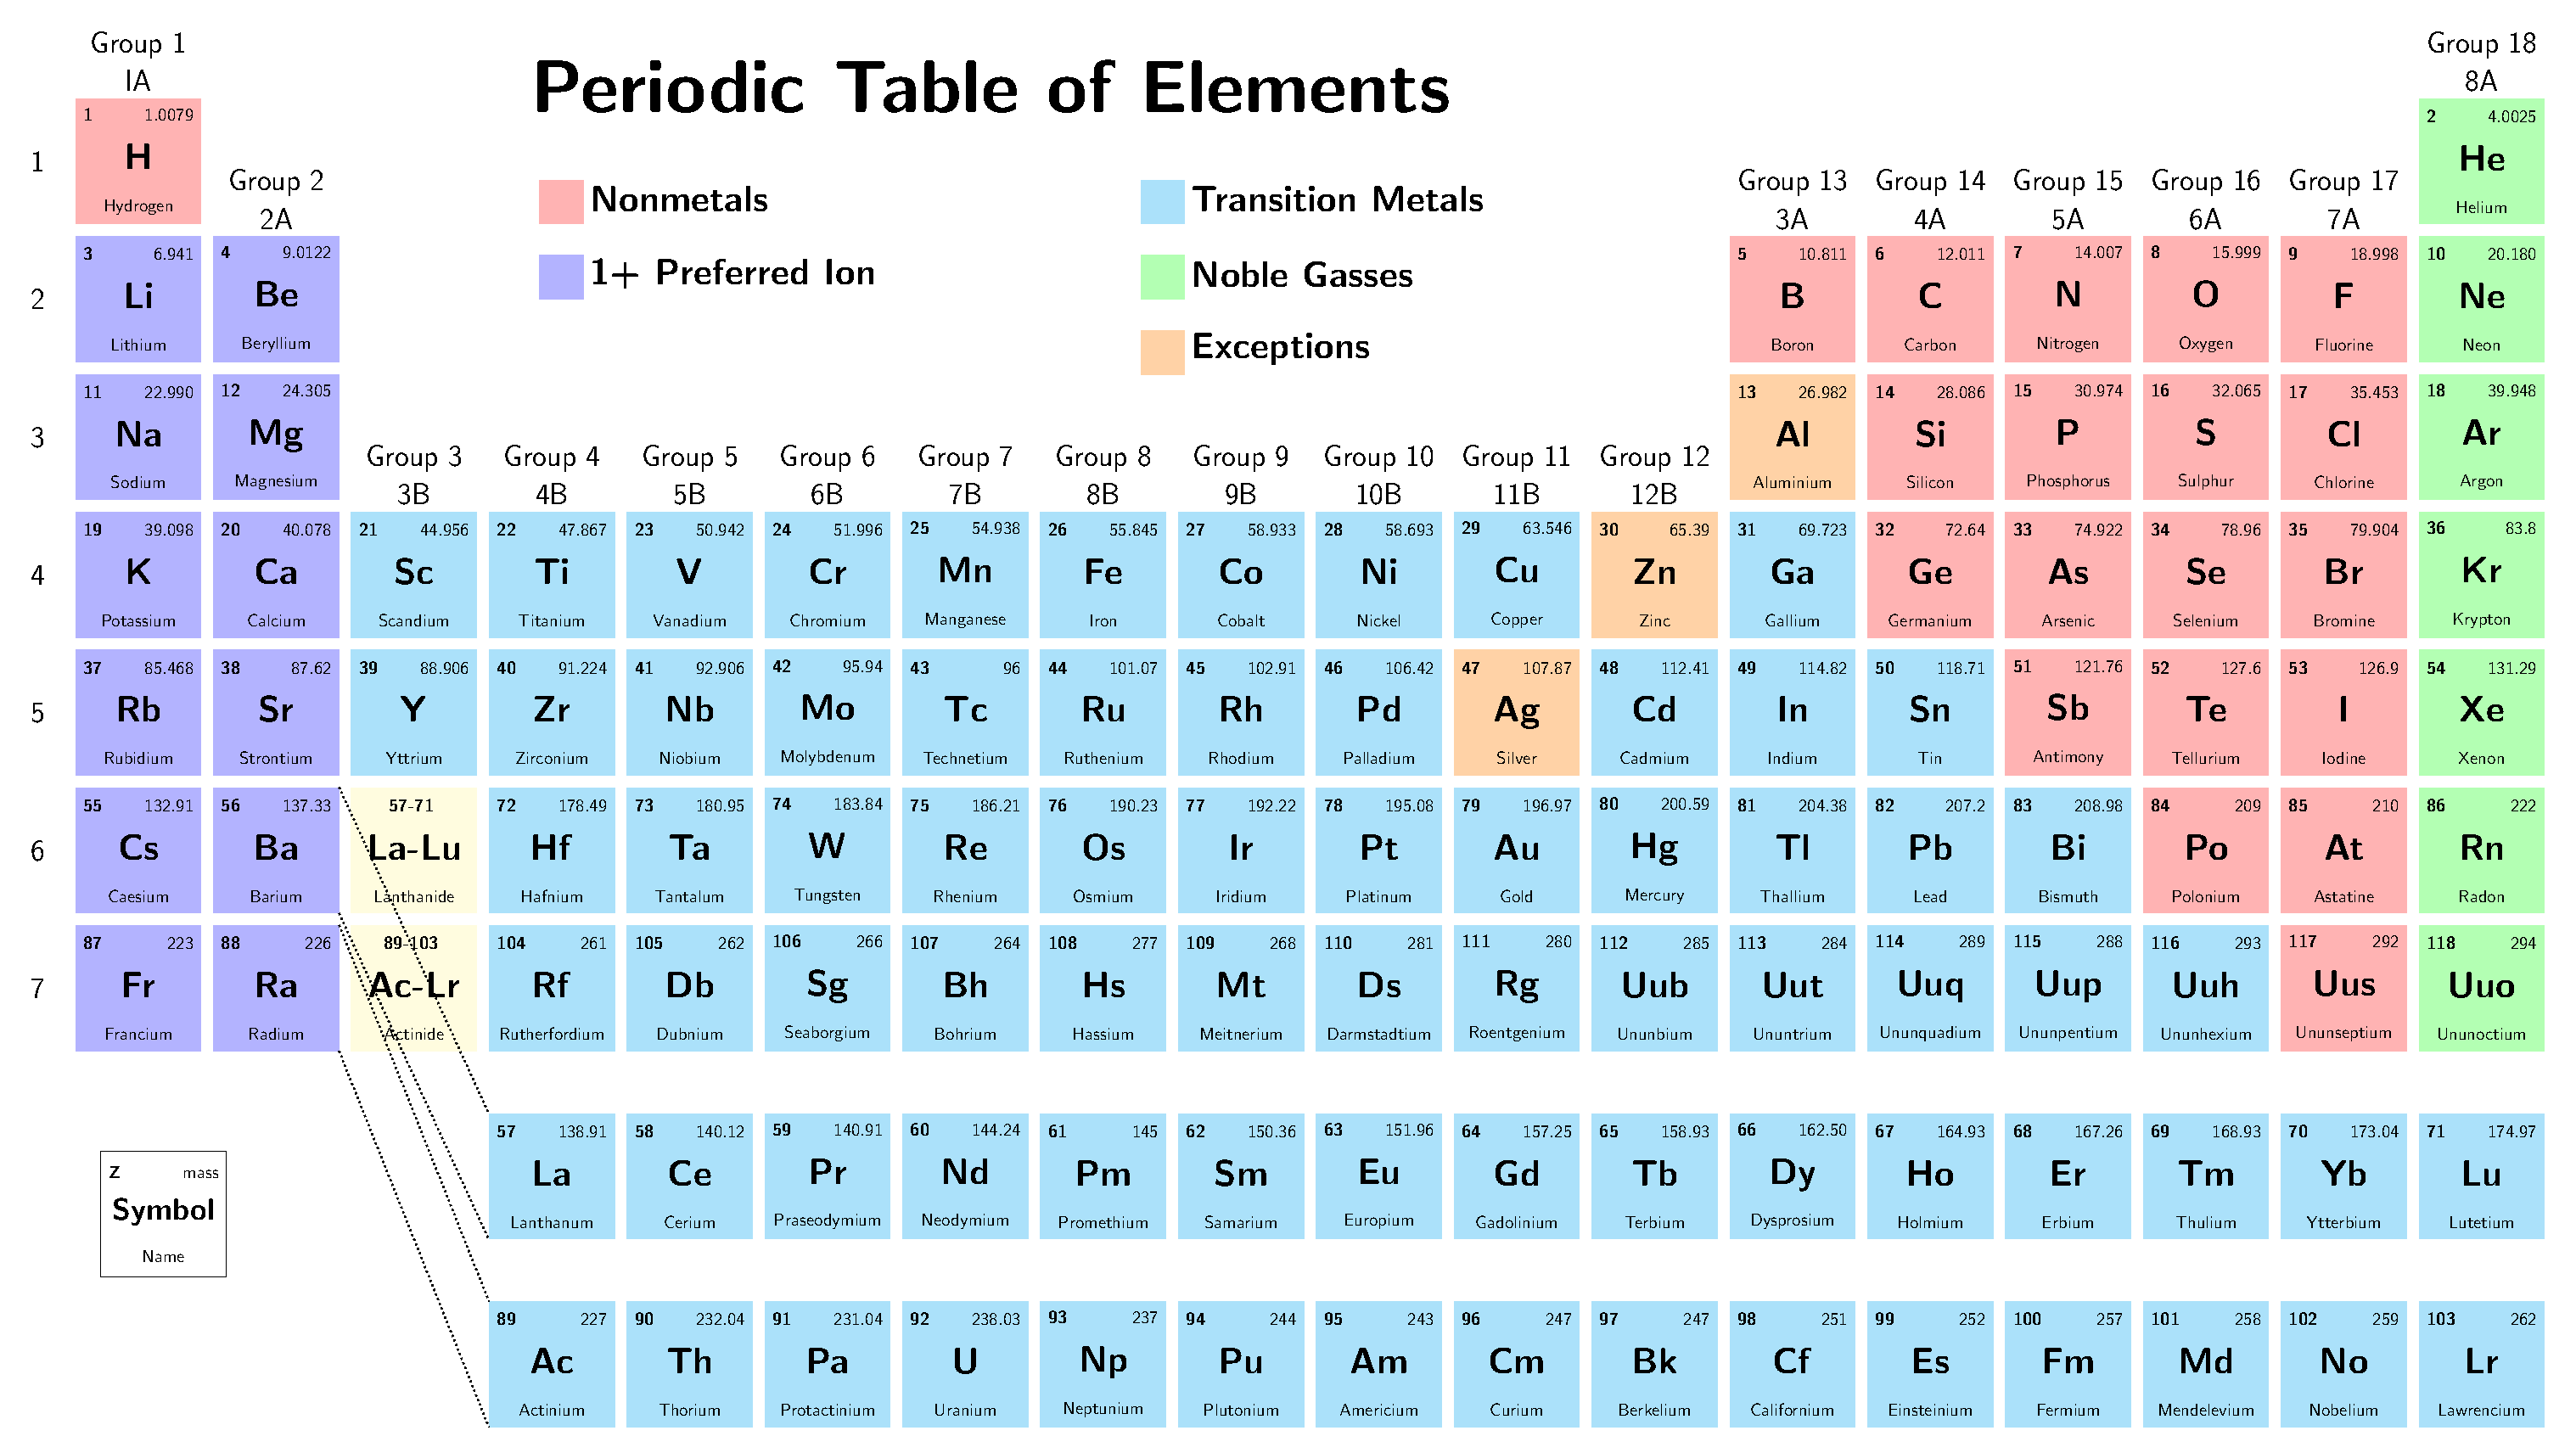
\includegraphics[width=1\linewidth]{PeriodicTableNamingRegions.pdf}
    \caption*{\textsl{\small{A periodic table recolored to separate elements into the categories used for chemical nomenclature. Nonmetals are red, metals are purple, transition metals are blue, noble gasses are green, and exceptions are orange.}}}
    \label{Periodic table colored into categories used for chemical nomenclature.}
\end{figure}

The more electronegative of the two elements will be named second and given the suffix -ide. This is similar to how ionic compounds are named when the anion is named in the same way. If the less electronegative element (the one named first) has only 1 atom present, the mono- prefix is usually omitted.

\begin{table}[H]
\centering
\begin{tabular}{ |c|c||c|c|} 
 \hline
 Prefix & Number & Prefix & Number\\ [0.5ex] 
 \hline\hline
 mono- & 1 & hexa- & 6\\ 
 \hline
 di- & 2 & hepta- & 7\\
 \hline
 tri- & 3 & octa- & 8\\
 \hline
 tetra- & 4 & nona- & 9\\
 \hline
 penta- & 5 & deca- & 10\\[1ex] 
 \hline
\end{tabular}
  \caption*{\textsl{\small{A table listing the prefixes used for one to 10 in chemical nomenclature}}}
\end{table}

A molecule made up of 2 Phosphorous atoms and 5 Oxygen atoms would have the chemical formula \ce{P2O5}. Phosphorous is less electronegative than Oxygen, so this compounds name is Diphosphorous Pentoxide.

A molecule made up of 1 Sulfur atom and 2 Oxygen atoms would have the chemical formula \ce{SO2}. Sulfur is less electronegative than Oxygen. There is only one Sulfur present, so the mono- prefix is omitted, so this compounds name is Sulfur Dioxide

\subsection{{\normalsize Ionic bonding: Nonmetal bound to a metal}}

This naming scheme applies when a metal from columns 1 or 2 is bound to a nonmetal(defined above). Both elements are treated as being their most stable ion. Column 1 and 2 metals form cations, and most nonmetals will form anions.

\begin{figure}[h]
    \centering
    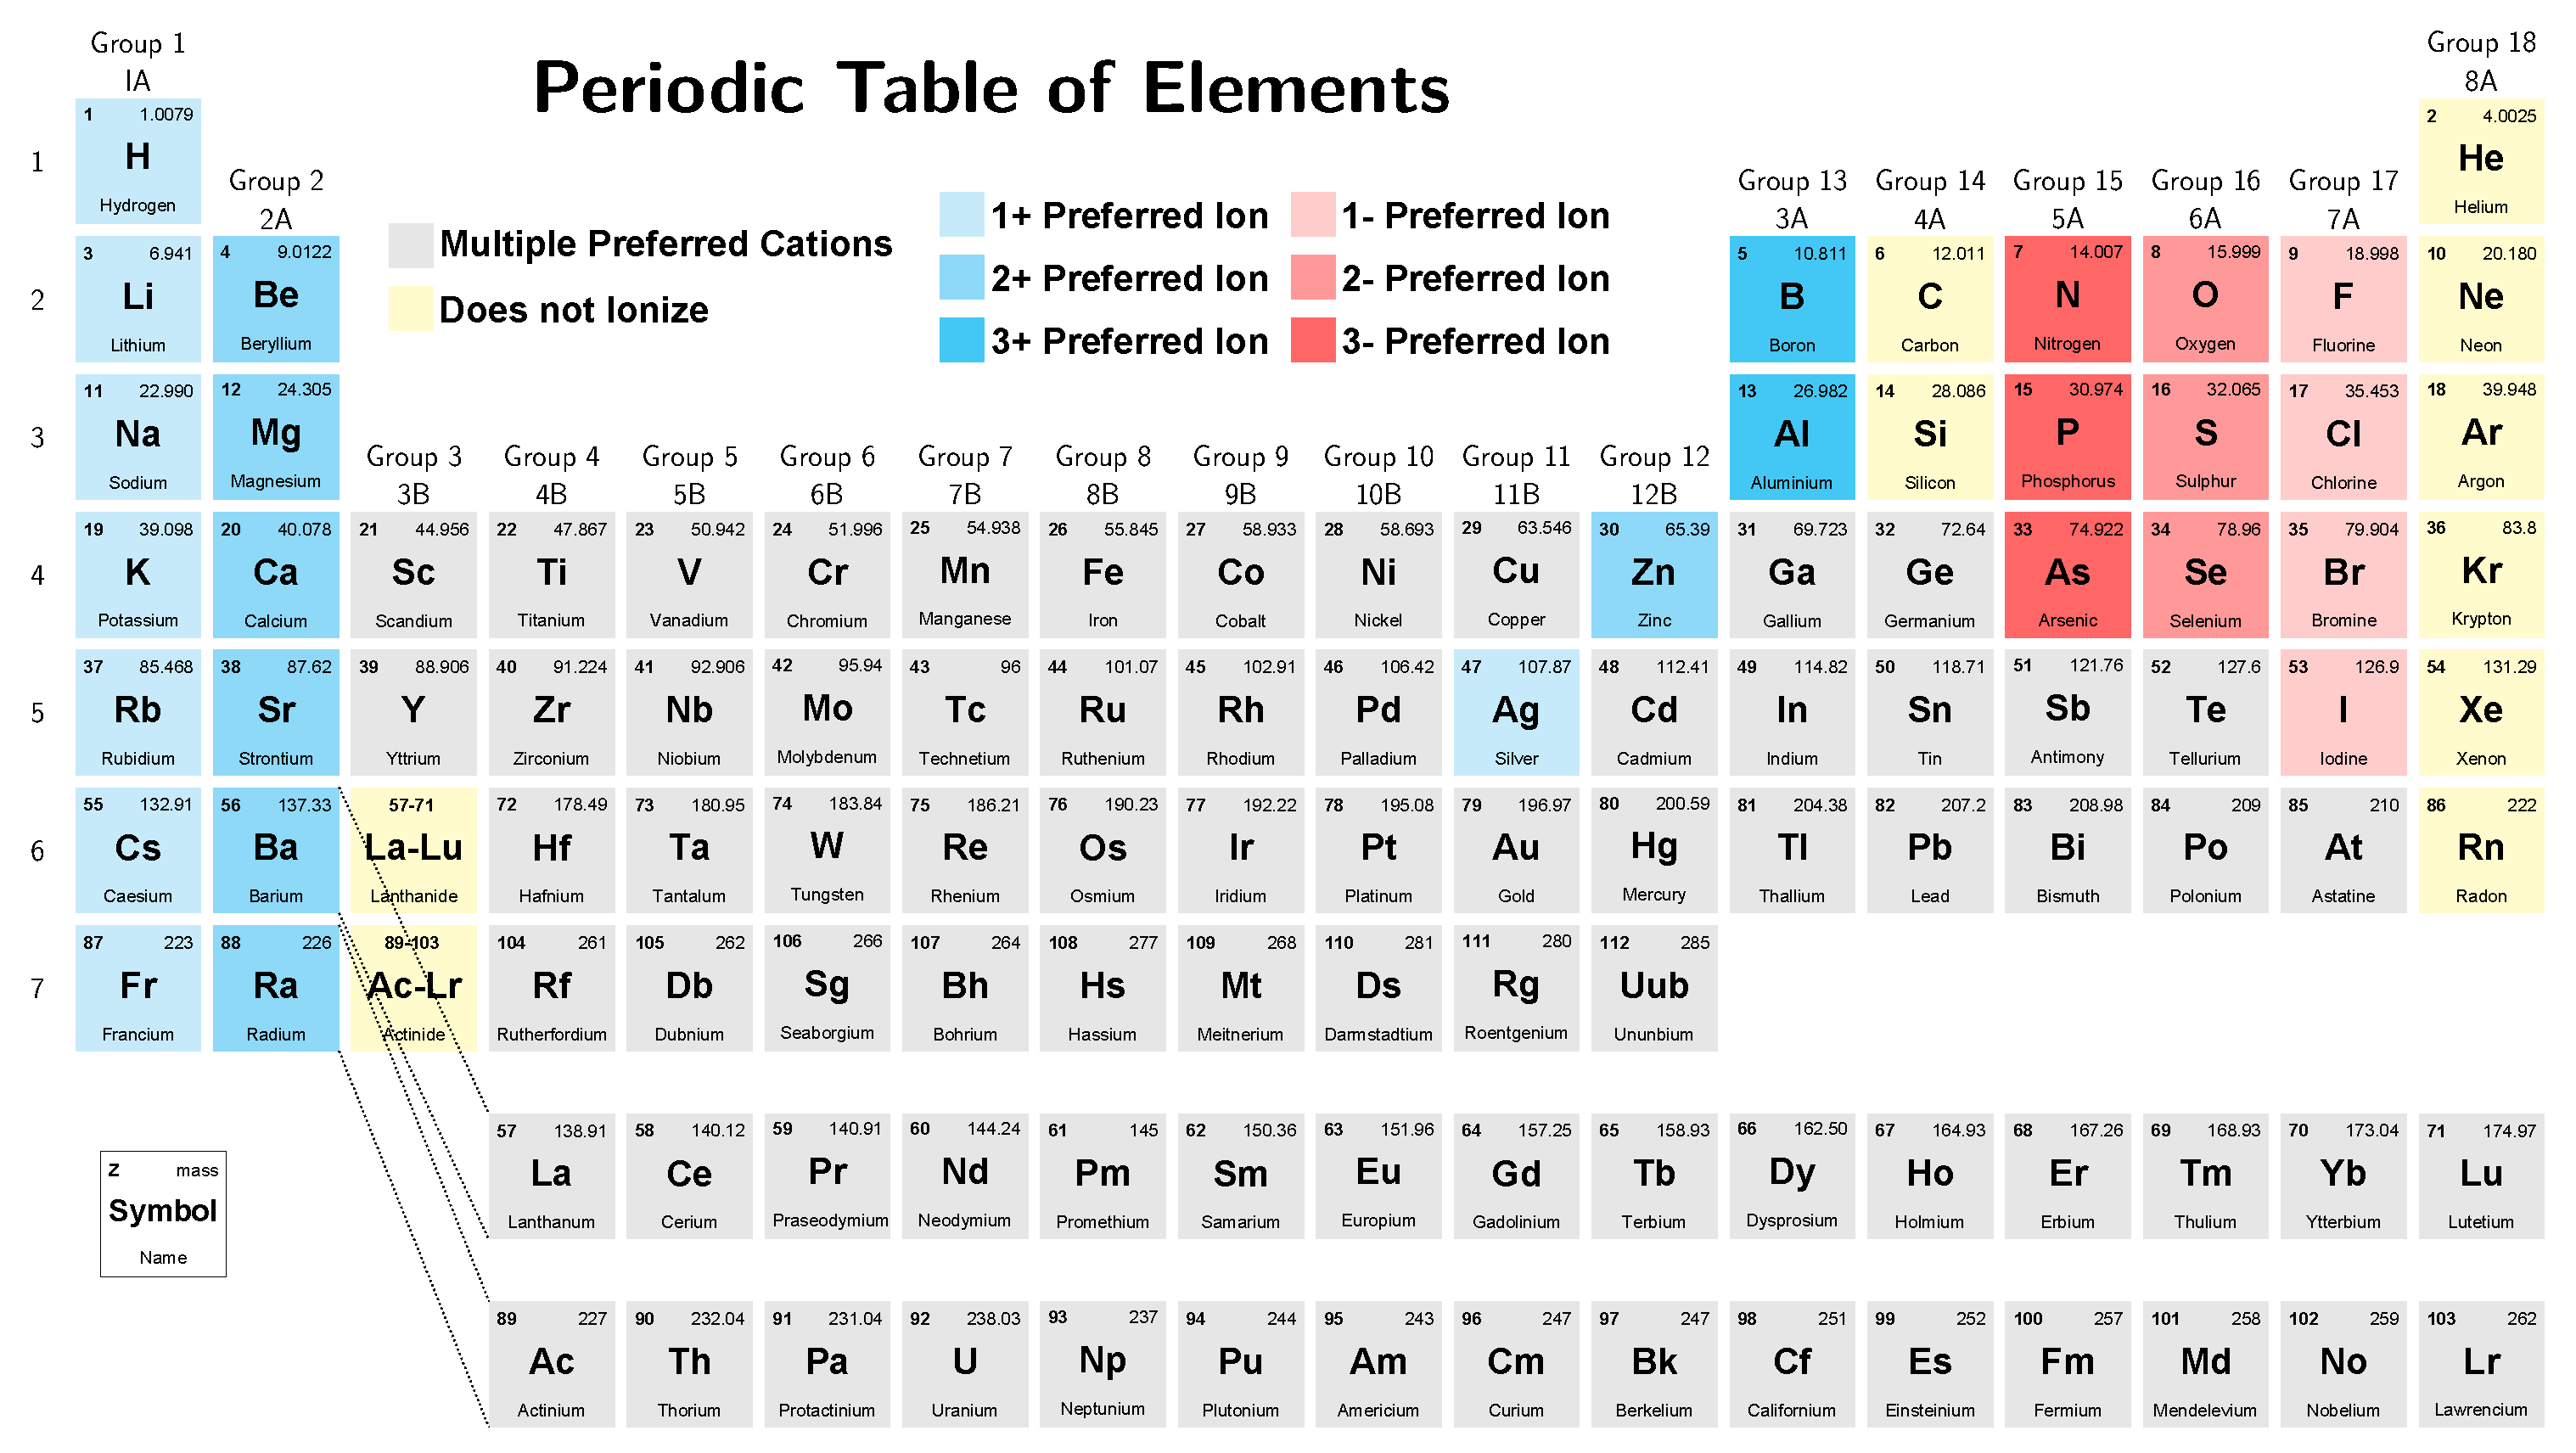
\includegraphics[width=1\linewidth]{PeriodicTableCommonIons.pdf}
    \caption*{\textsl{\small{A Periodic Table with each element colored to show its most common ion. Red elements form anions. Blue elements for cations. Darker shades of red or blue denote a larger magnitude of charge between 1 and 3. Gray elements can form multiple cations. Yellow elements very rarely ionize.}}}
    \label{Periodic table colored to show the most common ion made by each element}
\end{figure}

The magnitude of the charge depends on the elements valence electrons. An elements most stable ion will give the ion a noble gas configuration. The periodic table above shows the most stable ion formed by each element.


We can find this magnitude by thinking about how many "steps" away the element is from a noble gas. Flourine is one to the right away from the noble gas Neon, so its most stable ion wants to gain 1 electron and have a 1- charge. In fact, each element in the same column as Flourine is one step to the right away from a noble gas, so they will all prefer to form 1- anions. Nitrogen is 3 steps to the right away, so it would prefer to form a 3- anion. We can think of "stepping" off the left side of the periodic table as going to the noble gas in the previous row. Lithium and the rest of column 1 are each 1 step to the left away from a noble gas, so they would prefer to lose one electron and form 1+ cation. 

When naming ionic compounds, the number of atoms of each element is implied based on the most common ion each element will form. There are {\textbf not} prefixes denoting the number of atoms of each element like when naming covalent compounds. To determine the number of each ion present, find how many of each ion is needed to have a net charge of 0. 

Similar to covalent bonds, the less electronegative element (the cation) is named first. The more electronegative element (the anion) is named second with the -ide suffix. 

For example, the name for an ionic compound between Magnesium and Chlorine is Magnesium Chloride. The chemical formula is based on the most stable ions (\ce{Mg^2+} and \ce{Cl-}). Two Chloride ions are needed to cancel out the 2+ chargte on Magnesium, so the chemical formula is \ce{MgCl2}.

\newpage

\subsection{{\normalsize Compounds containing polyatomic ions}}

The naming conventions with polyatomic ions are nearly the same as with other ionic compounds. If the polyatomic ion is an anion, it is not given the -ide ending. 

In the chemical equation, the number of each ion is determined by how many of each are needed to have a net charge of 0. If multiple polyatomic ions are needed, the ion is placed in parentheses, and the subscript is placed after the parentheses. For the compound Magnesium Nitrate, two nitrate (\ce{NO3-}) ions are needed to neutralize \ce{Mg^2+}, so the chemical formula is written \ce{Mg(NO3)2}.

\subsection{{\normalsize Compounds containing transition metals}}

Transition metals are typically able to form multiple stable cations. They are named similar to ionic compounds, but name must communicate the oxidation state of the transition metal. The oxidation state is treated as a cation for determining names and chemical formulae. Oxidation states are written in Roman Numerals and placed in parentheses after the element name. The number of the metal and the anion are again determined by finding the number of each needed to have a net charge of 0. 

Iron(II) Chloride has Iron is the +2 oxidation state. The Iron is treated as having a +2 charge, so two Chlorides are needed to neutralize the charge. The chemical formula is \ce{FeCl2}.

\ce{FeCl3} is another stable compound between Iron and Chloride. This compound has an extra Chloride ion because Iron is in the +3 oxidation state. Therefore, \ce{FeCl3} is named Iron(III) chloride.  

\newpage

\section{{\normalsize Convert the chemical names below to chemical formulas.}} 
\vspace{10mm}


\flushleft{\textmd{a) Carbon Monoxide}}
\vspace{19mm}

\flushleft{\textmd{b) Phosphorous Pentoxide}}
\vspace{19mm}

\flushleft{\textmd{c) Magnesium Nitride}}
\vspace{19mm}

\flushleft{\textmd{d) Ammonium Phosphate}}
\vspace{19mm}

\flushleft{\textmd{e) Aluminum Sulfite}}
\vspace{19mm}

\flushleft{\textmd{f) Sodium Permanganate}}
\vspace{19mm}



\flushleft{\textmd{g) Carbon Tetrachloride}}
\vspace{19mm}

\flushleft{\textmd{h) Sodium Nitrate}}
\vspace{19mm}

\flushleft{\textmd{i) Titanium (IV) Oxide}}
\vspace{19mm}

\flushleft{\textmd{j) Magnesium Perchlorate}}
\vspace{19mm}

\flushleft{\textmd{k) Iron (III) Cyanide}}
\vspace{19mm}

\flushleft{\textmd{l) Aluminum Sulfate}}
\vspace{19mm}

\flushleft{\textmd{m) Magnesium Iodide}}
\vspace{19mm}

\flushleft{\textmd{n) Lead (II) Sulfate}}
\newpage

\section{{\normalsize Name the compounds below.}} 
\vspace{10mm}

\flushleft{\textmd{a) \ce{CO_2}}}
\vspace{19mm}

\flushleft{\textmd{b) \ce{OF2}}}
\vspace{19mm}

\flushleft{\textmd{c) \ce{P2O5}}}
\vspace{19mm}

\flushleft{\textmd{d) \ce{Al2(SO3)3}}}
\vspace{19mm}

\flushleft{\textmd{e) \ce{LiBr}}}
\vspace{19mm}

\flushleft{\textmd{f) \ce{CaCO3}}}
\vspace{19mm}

\flushleft{\textmd{g) \ce{Ag2CrO4}}}
\vspace{19mm}

\flushleft{\textmd{h) \ce{(NH4)3PO4}}}
\vspace{19mm}

\flushleft{\textmd{i) \ce{KCLO4}}}
\vspace{19mm}

\flushleft{\textmd{j) \ce{NaMnO4}}}
\vspace{19mm}

\flushleft{\textmd{k) \ce{Al(OH)3}}}
\vspace{19mm}

\flushleft{\textmd{l) \ce{AuCl3}}}
\vspace{19mm}

\flushleft{\textmd{m) \ce{TiO2}}}
\vspace{19mm}

\flushleft{\textmd{n) \ce{Pb3(PO4)4}}}

\end{document}

